% Options for packages loaded elsewhere
\PassOptionsToPackage{unicode}{hyperref}
\PassOptionsToPackage{hyphens}{url}
\PassOptionsToPackage{dvipsnames,svgnames,x11names}{xcolor}
%
\documentclass[
  12pt,
]{article}

\usepackage{amsmath,amssymb}
\usepackage{iftex}
\ifPDFTeX
  \usepackage[T1]{fontenc}
  \usepackage[utf8]{inputenc}
  \usepackage{textcomp} % provide euro and other symbols
\else % if luatex or xetex
  \usepackage{unicode-math}
  \defaultfontfeatures{Scale=MatchLowercase}
  \defaultfontfeatures[\rmfamily]{Ligatures=TeX,Scale=1}
\fi
\usepackage{lmodern}
\ifPDFTeX\else  
    % xetex/luatex font selection
\fi
% Use upquote if available, for straight quotes in verbatim environments
\IfFileExists{upquote.sty}{\usepackage{upquote}}{}
\IfFileExists{microtype.sty}{% use microtype if available
  \usepackage[]{microtype}
  \UseMicrotypeSet[protrusion]{basicmath} % disable protrusion for tt fonts
}{}
\makeatletter
\@ifundefined{KOMAClassName}{% if non-KOMA class
  \IfFileExists{parskip.sty}{%
    \usepackage{parskip}
  }{% else
    \setlength{\parindent}{0pt}
    \setlength{\parskip}{6pt plus 2pt minus 1pt}}
}{% if KOMA class
  \KOMAoptions{parskip=half}}
\makeatother
\usepackage{xcolor}
\usepackage[margin=1in]{geometry}
\setlength{\emergencystretch}{3em} % prevent overfull lines
\setcounter{secnumdepth}{-\maxdimen} % remove section numbering
% Make \paragraph and \subparagraph free-standing
\makeatletter
\ifx\paragraph\undefined\else
  \let\oldparagraph\paragraph
  \renewcommand{\paragraph}{
    \@ifstar
      \xxxParagraphStar
      \xxxParagraphNoStar
  }
  \newcommand{\xxxParagraphStar}[1]{\oldparagraph*{#1}\mbox{}}
  \newcommand{\xxxParagraphNoStar}[1]{\oldparagraph{#1}\mbox{}}
\fi
\ifx\subparagraph\undefined\else
  \let\oldsubparagraph\subparagraph
  \renewcommand{\subparagraph}{
    \@ifstar
      \xxxSubParagraphStar
      \xxxSubParagraphNoStar
  }
  \newcommand{\xxxSubParagraphStar}[1]{\oldsubparagraph*{#1}\mbox{}}
  \newcommand{\xxxSubParagraphNoStar}[1]{\oldsubparagraph{#1}\mbox{}}
\fi
\makeatother


\providecommand{\tightlist}{%
  \setlength{\itemsep}{0pt}\setlength{\parskip}{0pt}}\usepackage{longtable,booktabs,array}
\usepackage{calc} % for calculating minipage widths
% Correct order of tables after \paragraph or \subparagraph
\usepackage{etoolbox}
\makeatletter
\patchcmd\longtable{\par}{\if@noskipsec\mbox{}\fi\par}{}{}
\makeatother
% Allow footnotes in longtable head/foot
\IfFileExists{footnotehyper.sty}{\usepackage{footnotehyper}}{\usepackage{footnote}}
\makesavenoteenv{longtable}
\usepackage{graphicx}
\makeatletter
\newsavebox\pandoc@box
\newcommand*\pandocbounded[1]{% scales image to fit in text height/width
  \sbox\pandoc@box{#1}%
  \Gscale@div\@tempa{\textheight}{\dimexpr\ht\pandoc@box+\dp\pandoc@box\relax}%
  \Gscale@div\@tempb{\linewidth}{\wd\pandoc@box}%
  \ifdim\@tempb\p@<\@tempa\p@\let\@tempa\@tempb\fi% select the smaller of both
  \ifdim\@tempa\p@<\p@\scalebox{\@tempa}{\usebox\pandoc@box}%
  \else\usebox{\pandoc@box}%
  \fi%
}
% Set default figure placement to htbp
\def\fps@figure{htbp}
\makeatother
% definitions for citeproc citations
\NewDocumentCommand\citeproctext{}{}
\NewDocumentCommand\citeproc{mm}{%
  \begingroup\def\citeproctext{#2}\cite{#1}\endgroup}
\makeatletter
 % allow citations to break across lines
 \let\@cite@ofmt\@firstofone
 % avoid brackets around text for \cite:
 \def\@biblabel#1{}
 \def\@cite#1#2{{#1\if@tempswa , #2\fi}}
\makeatother
\newlength{\cslhangindent}
\setlength{\cslhangindent}{1.5em}
\newlength{\csllabelwidth}
\setlength{\csllabelwidth}{3em}
\newenvironment{CSLReferences}[2] % #1 hanging-indent, #2 entry-spacing
 {\begin{list}{}{%
  \setlength{\itemindent}{0pt}
  \setlength{\leftmargin}{0pt}
  \setlength{\parsep}{0pt}
  % turn on hanging indent if param 1 is 1
  \ifodd #1
   \setlength{\leftmargin}{\cslhangindent}
   \setlength{\itemindent}{-1\cslhangindent}
  \fi
  % set entry spacing
  \setlength{\itemsep}{#2\baselineskip}}}
 {\end{list}}
\usepackage{calc}
\newcommand{\CSLBlock}[1]{\hfill\break\parbox[t]{\linewidth}{\strut\ignorespaces#1\strut}}
\newcommand{\CSLLeftMargin}[1]{\parbox[t]{\csllabelwidth}{\strut#1\strut}}
\newcommand{\CSLRightInline}[1]{\parbox[t]{\linewidth - \csllabelwidth}{\strut#1\strut}}
\newcommand{\CSLIndent}[1]{\hspace{\cslhangindent}#1}

\usepackage{booktabs}
\usepackage{longtable}
\usepackage{array}
\usepackage{multirow}
\usepackage{wrapfig}
\usepackage{float}
\usepackage{colortbl}
\usepackage{pdflscape}
\usepackage{tabu}
\usepackage{threeparttable}
\usepackage{threeparttablex}
\usepackage[normalem]{ulem}
\usepackage{makecell}
\usepackage{xcolor}
\usepackage{setspace}
\usepackage{changepage}
\doublespacing
\makeatletter
\@ifpackageloaded{caption}{}{\usepackage{caption}}
\AtBeginDocument{%
\ifdefined\contentsname
  \renewcommand*\contentsname{Table of contents}
\else
  \newcommand\contentsname{Table of contents}
\fi
\ifdefined\listfigurename
  \renewcommand*\listfigurename{List of Figures}
\else
  \newcommand\listfigurename{List of Figures}
\fi
\ifdefined\listtablename
  \renewcommand*\listtablename{List of Tables}
\else
  \newcommand\listtablename{List of Tables}
\fi
\ifdefined\figurename
  \renewcommand*\figurename{Figure}
\else
  \newcommand\figurename{Figure}
\fi
\ifdefined\tablename
  \renewcommand*\tablename{Table}
\else
  \newcommand\tablename{Table}
\fi
}
\@ifpackageloaded{float}{}{\usepackage{float}}
\floatstyle{ruled}
\@ifundefined{c@chapter}{\newfloat{codelisting}{h}{lop}}{\newfloat{codelisting}{h}{lop}[chapter]}
\floatname{codelisting}{Listing}
\newcommand*\listoflistings{\listof{codelisting}{List of Listings}}
\makeatother
\makeatletter
\makeatother
\makeatletter
\@ifpackageloaded{caption}{}{\usepackage{caption}}
\@ifpackageloaded{subcaption}{}{\usepackage{subcaption}}
\makeatother

\usepackage{bookmark}

\IfFileExists{xurl.sty}{\usepackage{xurl}}{} % add URL line breaks if available
\urlstyle{same} % disable monospaced font for URLs
\hypersetup{
  pdftitle={Master Thesis - Outline and Results},
  colorlinks=true,
  linkcolor={blue},
  filecolor={Maroon},
  citecolor={Blue},
  urlcolor={Blue},
  pdfcreator={LaTeX via pandoc}}


\title{Master Thesis - Outline and Results}
\author{Rodrigo Dornelles}
\date{}

\begin{document}
\maketitle


\section{Introduction}\label{introduction}

\begin{itemize}
\item
  \textbf{The lack of legal empirical research:} Empirical legal
  research is still scarce, at least in Brazil. In the recent decades
  there were the idea of bringing a quantitative approach to Law, called
  jurimetrics Loevinger
  (\citeproc{ref-loevinger_jurimetricsnext_1948}{1948}). Recently, it is
  becoming more common to find studies based on empirical research as
  showed by Cabrera De Bonito et al.
  (\citeproc{ref-cabrera_de_bonito_pesquisa_2025}{2025}).
\item
  \textbf{SOTA of legal research}: Those studies, however, still uses
  little data from lawsuits and judicial precedents. Some of them do
  more qualitative/observational methods. To do more deep and broad
  analysis it is necessary to have a high level of resources and big and
  highly qualified research team. Examples of very good and important
  empirical research showed the relevant of this staff: Associação
  Brasileira de Jurimetria
  (\citeproc{ref-associacao_brasileira_de_jurimetria_avaliacao_2019}{2019}),
  Costa et al. (\citeproc{ref-costa_eficacia_2011}{2011}), Instituto de
  Pesquisa Econômica Aplicada (Ipea) \& Brasil. Ministério da Justiça e
  Segurança Pública
  (\citeproc{ref-instituto_de_pesquisa_economica_aplicada_ipea_perfil_2023}{2023}).
\item
  \textbf{Exploratory legal data analysis}: It is possible to simple
  analyze metadata of legal cases. Doing this would be useful to
  exploratory analysis and to formulate hypothesis. Data from lawsuits
  are also used as some examples shows. In Dornelles
  (\citeproc{ref-dornelles_o_2021}{2021}) data extracted from the
  Brazilian Supreme Court were used to describe the volume of new
  actions in the Court during Bolsonaro's administration:
\end{itemize}

\begin{figure}

{\centering \pandocbounded{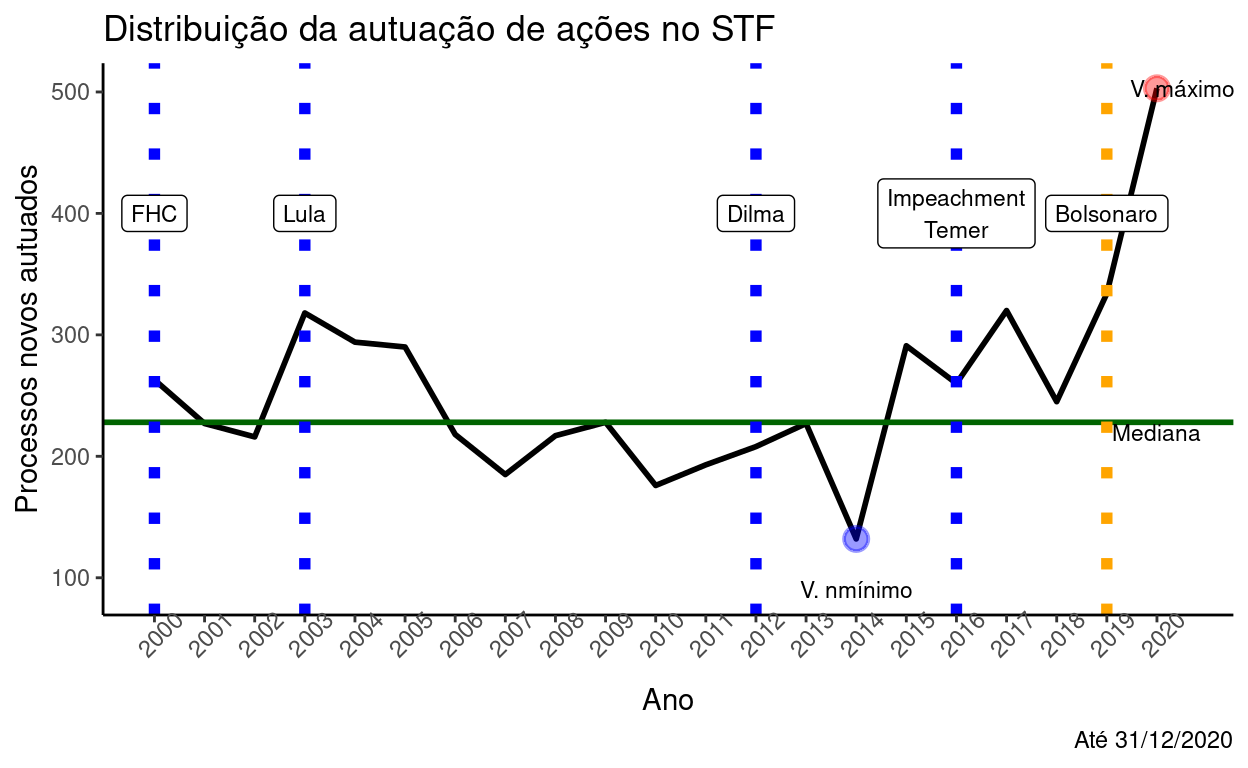
\includegraphics[keepaspectratio]{outline_files/mediabag/grafico_distribuicao.png}}

}

\caption{Evolution of new lawsuits each year in Brazilian Supreme Court.
Dornelles (\citeproc{ref-dornelles_o_2021}{2021})}

\end{figure}%

\begin{itemize}
\item
  \textbf{Robust research}: However, to do more legal research that goes
  beyond metadata. And, to do that, it is necessary to analyze complex
  documents in depth. Those documents are often relatively large and
  full of legal jargon, meaning that is also necessary that legal
  specialists do the analysis or, at least, oversee it.
\item
  \textbf{Natural Language Processing}: NLP is an important tool to
  handle text as data and to provide valuable insights from text
  documents. However, NLP models often are specialized in a single task
  Vajjala et al. (\citeproc{ref-vajjala_practical_2020}{2020}), while,
  to extract information from such documents it is necessary a handful
  of tools. Besides that, the traditional NLP models have little ability
  to understand larger contexts and to follow specific instructions
  Raschka (\citeproc{ref-raschka_build_2024}{2024}), so large language
  models would be a better approach to that. {[}\^{}1{]}.
\item
  \textbf{Opportunity}: The advent of powerful language models plus the
  high level of digitization of the Judiciary branch in Brazil would
  allow to a new era of empirical research, both into the academic and
  the practitioners perspective. It would be possible that a single
  researcher study how administrative misconduct law cases were decided
  and the last few years. Also, it would be possible to a Public
  Defender study Local Court's decisions in order to establish better
  strategy to new cases.
\item
  \textbf{This research}: The aim is to understand if and how large
  language models could be used to leverage legal research by processing
  whole judicial decisions and extracting the features of interest.
  Moreover, the interest is about understanding the feasibility to use
  open-source large language model in real-world settings.
\item
  \textbf{Open-source models}: In academia, in the public service and
  similar use cases, privacy and costs are a limitation. Although the
  terms of use of commercial LLMs might suggest a relative degree of
  confidence about data protection, once inserted in the API there is no
  real control over it. Also, the commercial models might be expensive
  (although cheaper than the fair price of human labor to do a similar
  task), which might be a block to its deployment.\footnote{Although
    there is some debate around Small Language Models and Large Language
    Models, this distinction is not being made here. See also Chen
    (\citeproc{ref-chen_empowering_2025}{2025})}
\end{itemize}

\section{Literature Review}\label{literature-review}

\begin{itemize}
\tightlist
\item
  \textbf{Brazilian legal research landscape}: Alves da Silva
  (\citeproc{ref-alves_da_silva_aspectos_2022}{2022}), Cabrera De Bonito
  et al. (\citeproc{ref-cabrera_de_bonito_pesquisa_2025}{2025})
\item
  \textbf{LLMs applied to legal field}: Junior et al.
  (\citeproc{ref-junior_juru_2024}{2024}), Katz et al.
  (\citeproc{ref-katz_natural_2023}{2023}), Bertalan \& Ruiz
  (\citeproc{ref-bertalan_predicting_nodate}{n.d.})
\item
  \textbf{LLMs in Portuguese}: Niklaus et al.
  (\citeproc{ref-niklaus_multilegalpile_2023}{2023}), Almeida et al.
  (\citeproc{ref-almeida_sabia-2_2024}{2024}), Pires et al.
  (\citeproc{ref-pires_sabia_2023}{2023})
\item
  \textbf{Specialization in Legal Tasks}: This is the paper that most
  gave actionable inputs to this research: Dominguez-Olmedo et al.
  (\citeproc{ref-dominguez-olmedo_lawma_2024}{2024})
\end{itemize}

\section{Research Question}\label{research-question}

Can open-source large language models be deployed in the Brazilian legal
context to accurately extract information, recognize entities, and
summarize complex legal documents?

\section{Data}\label{data}

\begin{itemize}
\tightlist
\item
  \textbf{Lacerda Dataset}: Lacerda e Silva
  (\citeproc{ref-lacerda_e_silva_punindo_2021}{2021}) did a
  comprehensive empirical analysis on over 400 legal cases related to
  drug traffic. She gathered those cases in São Paulo's State Court of
  Justice (TJSP) in a sample covering between 2017 to 2018 and she
  annotated and labelled about 35 features of each case manually. I
  received the data from the researcher and adapted the dataset to this
  research.
\end{itemize}

Some of the original features also referred to other documents rather
than the judicial decision and, therefore, they were excluded (since it
would not be reasonable that the model inferred that). Also, features
that were related to biological data were excluded due ethical reasons.

Also, I have tried to access Instituto de Pesquisa Econômica Aplicada
(Ipea) \& Brasil. Ministério da Justiça e Segurança Pública
(\citeproc{ref-instituto_de_pesquisa_economica_aplicada_ipea_perfil_2023}{2023})
micro data to build a golden dataset since they have about 3.5k data
points labelled. I have filled a freedom of information request and,
although it was possible to access the
\href{https://www.gov.br/mj/pt-br/assuntos/sua-protecao/politicas-sobre-drogas/pesquisa-e-informacao-3/pesquisa\%20IPEA/pesquisa-ipea-perfil-processado-e-producao-de-provas}{general
dataset}, they have not provided the lawsuit identifier, so it was not
possible to match each row in their dataset to a legal case and,
therefore, to a specific document.

\begin{itemize}
\item
  \textbf{Judicial Decisions}: The documents relative to each decision
  case analyzed by the Lacerda Dataset were extracted automatically from
  the TJSP website. Since there is no API to that, the process was done
  using Filho \& Trecenti (\citeproc{ref-filho_coleta_2020}{2020})
  package called \{tjsp\}. It gathered metadata of each case and the
  decision in string format in a R dataframe. Some cases where collected
  by its .pdf files and read automatically.
\item
  \textbf{Final dataset}: After the cleaning process, some duplication
  were excluded and some documents were not collected, the final result
  was a dataset with 258 cases. Also, the final dataset contained 50
  columns: it was due some categorical features were transformed in
  boolean. For instance: the column \emph{DenDrogas} contained
  information about the most common articles of law that were in the
  accusation. It was transformed in the columns:
  \emph{denuncia\_art\_33}, \emph{denuncia\_art\_34} and
  \emph{denuncia\_art\_35}.
\end{itemize}

\section{Theoretical Framework}\label{theoretical-framework}

\begin{itemize}
\tightlist
\item
  \textbf{Natural Language Processing}
\item
  \textbf{LLMs}
\item
  \textbf{Fine tuning}: Using Dominguez-Olmedo et al.
  (\citeproc{ref-dominguez-olmedo_lawma_2024}{2024}) strategy.
\end{itemize}

\section{Models}\label{models}

We used 12 models in this research. Models from OpenAI were considered
commercials and the others open source. Also, OpenAI do not disclose
their architectures, so it is not possible to know beforehand their
number of parameters.

\begin{longtable*}[t]{llll}
\toprule
model & family & parameters & type\\
\midrule
GPT 4.1 & OpenAI & unknown & commercial\\
GPT 4.1-mini & OpenAI & unknown & commercial\\
GPT 4.1-nano & OpenAI & unknown & commercial\\
GPT 4o & OpenAI & unknown & commercial\\
GPT 4o-mini & OpenAI & unknown & commercial\\
\addlinespace
o3-mini & OpenAI & unknown & commercial\\
Gemma 3 & Gemma & 27 B & open-source\\
Gemma 3 & Gemma & 12 B & open-source\\
Gemma 3 & Gemma & 1 B & open-source\\
Llama 3.1 & Llama & 8 B & open-source\\
\addlinespace
Llama 3.2 & Llama & 3 B & open-source\\
Phi 4 & Phi & 14 B & open-source\\
Lawma 8B & Lawma & 8 B & open-source\\
Tucano & Tucano & 2.4 B & open-source\\
\bottomrule
\end{longtable*}

\section{Methods}\label{methods}

\begin{itemize}
\tightlist
\item
  etl
\item
  prompt engeneenering, build schema
\item
  generation in OpenAI's models
\item
  evaluation pipeline
\item
  generation with commercial models

  \begin{itemize}
  \tightlist
  \item
    window context: rope scaling, yarn, rag, chuncking
  \item
    structured output
  \item
    base model generation
  \end{itemize}
\item
  finetune commercial and open source models

  \begin{itemize}
  \tightlist
  \item
    OpenAI's API
  \item
    Unsloth
  \end{itemize}
\item
  final evaluation
\end{itemize}

\section{Results}\label{results}

After 17 experiments\footnote{Ignoring validation tests and the
  experiences to try to overcome the limitations regarding context
  windows. Also, in this count there were the fine tune.}, it was
possible to gather the metrics above regarding accuracy. By accuracy we
are considering the proportion of exact answers regarding the total
answers. Bellow, we can see the performance of the base models, before
fine tuning.

\begin{longtable*}[t]{llllr}
\toprule
family & type & model & parameters & accuracy\\
\midrule
Gemma & open-source & Gemma 3 & 27 B & 0.8200\\
OpenAI & commercial & GPT 4o & unknown & 0.7878\\
OpenAI & commercial & o3-mini & unknown & 0.7638\\
Gemma & open-source & Gemma 3 & 12 B & 0.7627\\
OpenAI & commercial & GPT 4.1 & unknown & 0.7545\\
\addlinespace
Phi & open-source & Phi 4 & 14 B & 0.7474\\
Llama & open-source & Llama 3.1 & 8 B & 0.7354\\
OpenAI & commercial & GPT 4o-mini & unknown & 0.7114\\
OpenAI & commercial & GPT 4.1-mini & unknown & 0.6967\\
OpenAI & commercial & GPT 4.1-nano & unknown & 0.6590\\
\addlinespace
Llama & open-source & Llama 3.2 & 3 B & 0.5423\\
Gemma & open-source & Gemma 3 & 1 B & 0.0000\\
\bottomrule
\end{longtable*}

The model Gemma 3-1B achieved 0.0 accuracy due their lack of abilities
to yield structured JSON outputs.

The model that best performed in a zero-shot approach was the Gemma
3-27B parameters, which, surprisingly, also beat the benchmark
commercial models, even GPT-4o. Also, the Gemma 3 family seems to be
very prone to yield accurate results, since the lighter version with 12B
parameter also performed very well and was better than the newly
released GPT-4.1. The model Phi-4 performed also very well, also betting
OpenAI's smaller models. Regarding the Llama family, the 3.1 version
performed better than 4o-mini and the smallers GPT 4.1-mini and GPT
4.1-nano. On the other hand, Llama 3.2 had a bad performance.

Trying to understand a more fine-grained analysis, it was possible to
break the results by the kind of taks. The \emph{numeric} tasks are
those related to extract and calculate the amount of drugs or the prison
time in months: those tasks involved not only recognizing the numbers
(entities) but also to `calculate' the final value. The \emph{boolean}
tasks are generally in the realm of question answering in a
TRUE/FALSE/None style (for instance, if the art. 33 was the basis of the
sentence or if there were confession by the defendant). The
\emph{categorical} tasks are those closely related to classification
tasks, such as what was the outcome of the case (conviction, acquittal,
etc.). The \emph{open textual} tasks are more likely to be similar to
named entity recognition: in this case, the name of the Judge and the
defendant.

\pandocbounded{
\includegraphics[keepaspectratio]{../../evaluate_results/task_accuracy_heatmap.png}}
We can see that the \emph{open textual} tasks have a very high level of
performance in nearly all models, while the boolean and categorical
tasks were more diverse performance-wise. We can se also some
differences in numeric tasks, but in general they all performed very
well.

Those results suggested that keep working with open source models were a
promising strategy. So fine tuning was performed with the models OpenAI
4o-mini (which is the recommended model by OpenAI), Llama 3.2 (3B) and
Phi4. There were no resources available to perform fine tune on other
models. After the fine tuning, we could see a big improvement in the
results.

\begin{figure}

{\centering \pandocbounded{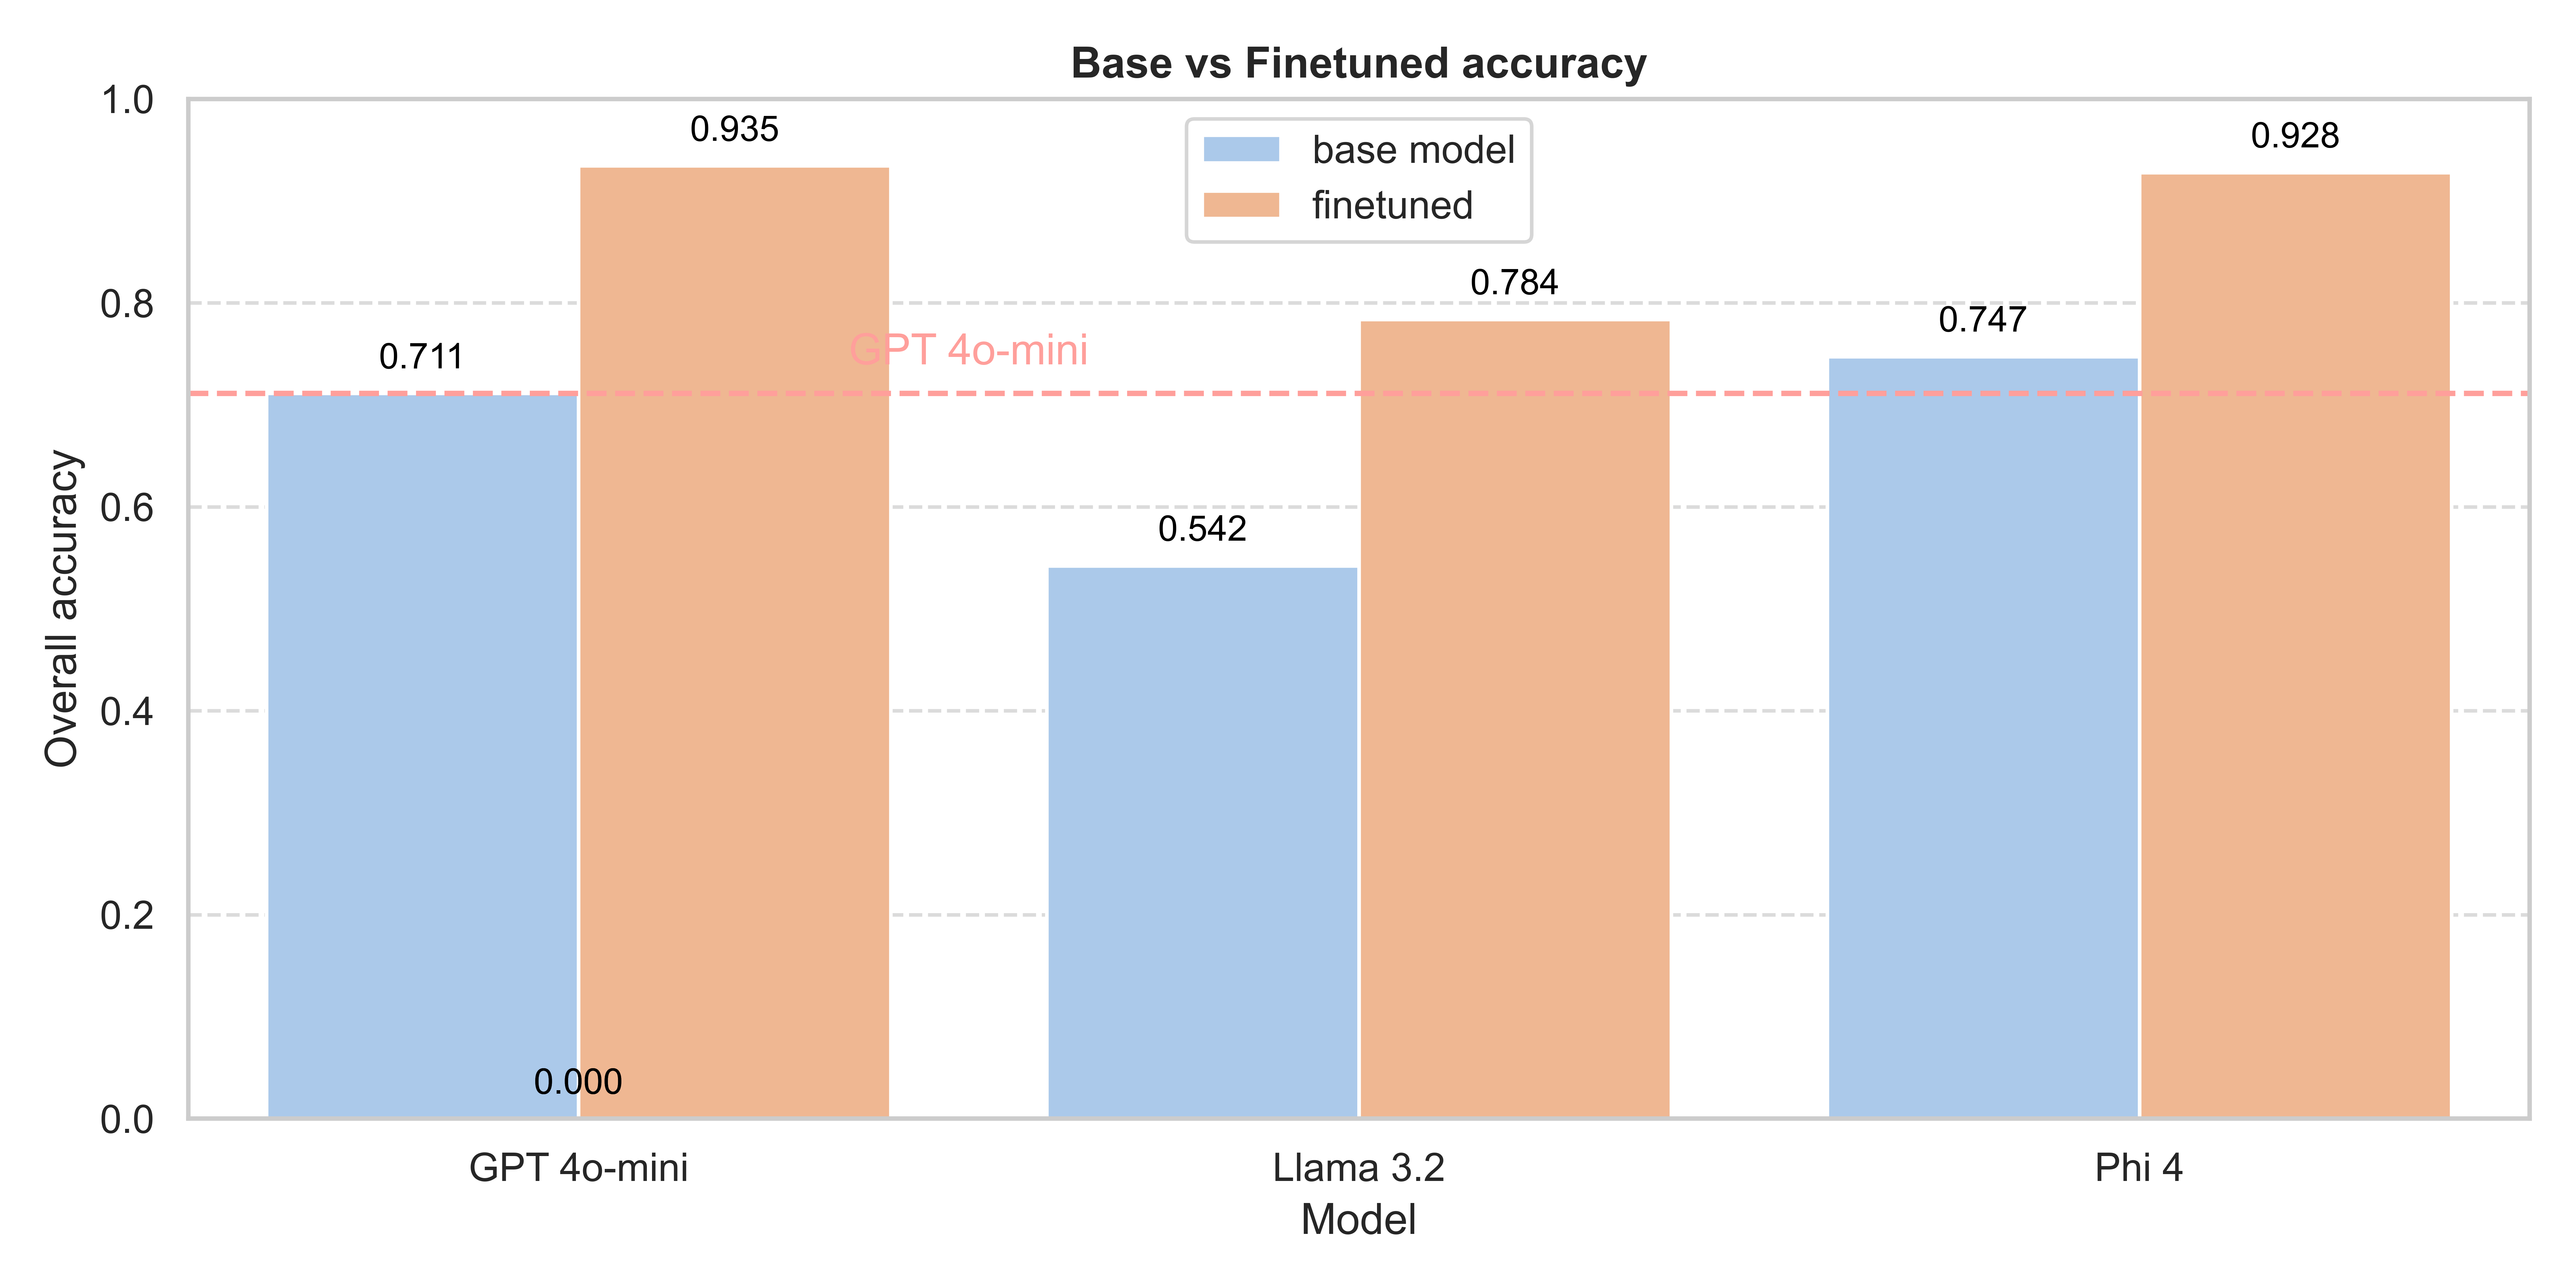
\includegraphics[keepaspectratio]{../../evaluate_results/base_vs_finetuned_accuracy.png}}

}

\caption{Models after fine tuning}

\end{figure}%

The process of fine tuning, even with a small dataset with 186 cases,
highly improved the performance of the models, confirming the `power of
specialization' as suggested by
(\citeproc{ref-dominges_olmedo_lawma_2024}{\textbf{dominges\_olmedo\_lawma\_2024?}}).
As (\citeproc{ref-fig:finetune}{\textbf{fig:finetune?}}) showed, model
Phi4 tied with GPT 4o-mini and the much smaller Llama 3.2 (3B) learnt
very easily in the process, even both models being trained with the same
10 epochs. It suggests that with a richer dataset and/or more epochs it
would be possible to reach or even surpass GPT 4o-mini performance.

\begin{longtable}[t]{lrrr}

\toprule
metric & GPT 4o-mini & Llama 3.2 & Phi 4\\
\midrule
Δ accuracy & 0.22 & 0.24 & 0.18\\
\% accuracy & 31.37 & 44.57 & 24.16\\
Δ boolean & 0.29 & 0.20 & 0.21\\
\% boolean & 43.56 & 34.54 & 28.63\\
Δ categorical & -0.04 & 0.48 & 0.14\\
\addlinespace
\% categorical & -4.46 & 145.31 & 17.76\\
Δ numeric & 0.11 & 0.28 & 0.09\\
\% numeric & 14.44 & 62.15 & 11.17\\
Δ open textual & 0.01 & 0.21 & 0.08\\
\% open textual & 1.35 & 33.00 & 8.82\\
\bottomrule


\caption{\label{tbl-finetune-delta}Fine tuned models: change in accuracy
(absolute value Δ and relative value \%)}

\tabularnewline
\end{longtable}

As Table~\ref{tbl-finetune-delta} shows, Llama 3.2(3B) had the highest
change in is performance, specially with the categorical tasks.
Specifically with this kind of tasks, we could see a degradation of
performance of GPT 4o-mini. Phi4, al\footnote{There is the
  \href{https://huggingface.co/microsoft/Phi-4-mini-instruct}{mini
  version of Phi-4}, however it was not possible to run or fine tune it
  with the actual computational resources.}though had the second-best
performance, learnt relatively less than Llama which might suggest a
ceiling. Assuming that, in those architectures, the number of parameters
is the critical factor, maybe less parameters than 14B and more than 3B
would be ideal.

\section{Policy Recommendations}\label{policy-recommendations}

\begin{itemize}
\item
  Academia: disclose data from empirical legal research as much as
  possible, as it would be valuable resource to fine tune models. If
  IPEA released the data from Instituto de Pesquisa Econômica Aplicada
  (Ipea) \& Brasil. Ministério da Justiça e Segurança Pública
  (\citeproc{ref-instituto_de_pesquisa_economica_aplicada_ipea_perfil_2023}{2023}),
  would it be possible to achieve even better results.
\item
  Open source community: keep the standard of at least 128k context
  window and develop light open source models. Wolf et al.
  (\citeproc{ref-wolf_transformers_2020}{2020}) is a very important
  framework to training and inference. Daniel Han \& team
  (\citeproc{ref-daniel_han_unsloth_2023}{2023}) was valuable to
  efficiently fine tune models efficiently.
\item
  Judiciary branch: make sure data and documents from lawsuits are
  available digitally for research, keeping high standards of privacy.
  It would be feasible through anonymization.
\item
  Instituions interested in empirical legal research: the balance of
  easiness and performance are probably better with OpenAI's API. But
  open source models showed to be powerful to this tasks and might be
  deployed to accelerate empirical research in Law.
\item
  Law schools: invest in data literacy to legal students and
  practitioners.
\end{itemize}

\section{References}\label{references}

\phantomsection\label{refs}
\begin{CSLReferences}{1}{0}
\bibitem[\citeproctext]{ref-almeida_sabia-2_2024}
Almeida, T. S., Abonizio, H., Nogueira, R., \& Pires, R. (2024).
\emph{Sabiá-2: {A} {New} {Generation} of {Portuguese} {Large} {Language}
{Models}}. arXiv. \url{https://doi.org/10.48550/arXiv.2403.09887}

\bibitem[\citeproctext]{ref-alves_da_silva_aspectos_2022}
Alves da Silva, P. E. (2022). Aspectos metodológicos da pesquisa
empírica em {Direito} com processos judiciais físicos e eletrônicos. In
\emph{Estudos empíricos em processo e organização judiciária}. Expert.

\bibitem[\citeproctext]{ref-associacao_brasileira_de_jurimetria_avaliacao_2019}
Associação Brasileira de Jurimetria. (2019). \emph{Avaliação do
{Impacto} de {Critérios} {Objetivos} na {Distinção} {Entre} {Posse} para
{Uso} e {Posse} para {Tráfico}: {Um} estudo {Jurimétrico}}. Associação
Brasileira de Jurimetria.
\url{https://abj.org.br/pdf/20190402_abj_criterios_objetivos.pdf}

\bibitem[\citeproctext]{ref-bertalan_predicting_nodate}
Bertalan, V. G. F., \& Ruiz, E. E. S. (n.d.). \emph{Predicting
{Judicial} {Outcomes} in the {Brazilian} {Legal} {System} {Using}
{Textual} {Features}}.

\bibitem[\citeproctext]{ref-cabrera_de_bonito_pesquisa_2025}
Cabrera De Bonito, B., Veloso De Castro, C., \& Korasaki, V. (2025).
{PESQUISA} {QUANTITATIVA} {NO} {DIREITO}: {UMA} {REVISÃO}
{BIBLIOGRÁFICA}. \emph{Revista de Estudos Empíricos Em Direito},
\emph{11}. \url{https://doi.org/10.19092/reed.v11.830}

\bibitem[\citeproctext]{ref-chen_empowering_2025}
Chen, W. (2025). Empowering innovation: {The} next generation of the
{Phi} family. In \emph{Microsoft Azure Blog}.
\url{https://azure.microsoft.com/en-us/blog/empowering-innovation-the-next-generation-of-the-phi-family/}

\bibitem[\citeproctext]{ref-costa_eficacia_2011}
Costa, S. H. da, Silva, P. E. A. da, Sabino, M. A. da C., Fernandes, D.
C. M., \& Lusvarghi, L. A. dos S. (2011). \emph{A eficácia do sistema
jurídico de prevenção e combate à improbidade administrativa}
{[}Publicação de relatório de pesquisa{]}. Secretaria de Assuntos
Legislativos do Ministério da Justiça.
\url{https://web.archive.org/web/20211004195943/http://pensando.mj.gov.br/wp-content/uploads/2015/07/34Pensando_Direito1.pdf}

\bibitem[\citeproctext]{ref-daniel_han_unsloth_2023}
Daniel Han, M. H., \& team, U. (2023). \emph{Unsloth}.
\url{http://github.com/unslothai/unsloth}

\bibitem[\citeproctext]{ref-dominguez-olmedo_lawma_2024}
Dominguez-Olmedo, R., Nanda, V., Abebe, R., Bechtold, S., Engel, C.,
Frankenreiter, J., Gummadi, K., Hardt, M., \& Livermore, M. (2024).
\emph{Lawma: {The} {Power} of {Specialization} for {Legal} {Tasks}}.
arXiv. \url{http://arxiv.org/abs/2407.16615}

\bibitem[\citeproctext]{ref-dornelles_o_2021}
Dornelles, R. F. (2021). O {STF}, o controle concentrado e a pandemia.
In \emph{Associação Brasileira de Jurimetria}.
\url{https://lab.abj.org.br/posts/2021-04-13-stf-controle-concentrado/}

\bibitem[\citeproctext]{ref-filho_coleta_2020}
Filho, J. de J., \& Trecenti, J. (2020). \emph{Coleta e organização de
dados do {Tribunal} de {Justiça} de {São} {Paulo}}.
\url{https://jjesufilho.github.io/tjsp/}

\bibitem[\citeproctext]{ref-instituto_de_pesquisa_economica_aplicada_ipea_perfil_2023}
Instituto de Pesquisa Econômica Aplicada (Ipea), \& Brasil. Ministério
da Justiça e Segurança Pública. (2023). \emph{Perfil do processado e
produção de provas nas ações criminais por tráfico de drogas : Relatório
analítico nacional dos {Tribunais} {Estaduais} de {Justiça} {Comum}}.
Instituto de Pesquisa Econômica Aplicada (Ipea).
\url{https://doi.org/10.38116/ri221151}

\bibitem[\citeproctext]{ref-junior_juru_2024}
Junior, R. M., Pires, R., Romero, R., \& Nogueira, R. (2024).
\emph{Juru: {Legal} {Brazilian} {Large} {Language} {Model} from
{Reputable} {Sources}}. arXiv.
\url{https://doi.org/10.48550/arXiv.2403.18140}

\bibitem[\citeproctext]{ref-katz_natural_2023}
Katz, D. M., Hartung, D., Gerlach, L., Jana, A., \& II, M. J. B. (2023).
\emph{Natural {Language} {Processing} in the {Legal} {Domain}}. arXiv.
\url{https://doi.org/10.48550/arXiv.2302.12039}

\bibitem[\citeproctext]{ref-lacerda_e_silva_punindo_2021}
Lacerda e Silva, M. (2021). \emph{Punindo as diferenças: {Gênero}, raça
e geração no sentenciamento de tráfico de drogas na cidade de {São}
{Paulo}}. \url{http://repositorio.unb.br/handle/10482/41413}

\bibitem[\citeproctext]{ref-loevinger_jurimetricsnext_1948}
Loevinger, L. (1948). Jurimetrics--{The} {Next} {Step} {Forward}.
\emph{Minn. L. Rev.}, \emph{33}, 455.

\bibitem[\citeproctext]{ref-niklaus_multilegalpile_2023}
Niklaus, J., Matoshi, V., Sturmer, M., Chalkidis, I., \& Ho, D. E.
(2023). \emph{{MultiLegalPile}: {A} {689GB} {Multilingual} {Legal}
{Corpus}}. \url{https://doi.org/10.48550/arXiv.2306.02069}

\bibitem[\citeproctext]{ref-pires_sabia_2023}
Pires, R., Abonizio, H., Almeida, T. S., \& Nogueira, R. (2023).
\emph{Sabiá: {Portuguese} {Large} {Language} {Models}} (Vol. 14197, pp.
226--240). \url{https://doi.org/10.1007/978-3-031-45392-2_15}

\bibitem[\citeproctext]{ref-raschka_build_2024}
Raschka, S. (2024). \emph{Build a {Large} {Language} {Model} (from
{Scratch})}. Manning Publications Co. LLC.
\url{http://ebookcentral.proquest.com/lib/hertie-school/detail.action?docID=31657639}

\bibitem[\citeproctext]{ref-vajjala_practical_2020}
Vajjala, S., Majumder, B., Gupta, A., \& Surana, H. (2020).
\emph{Practical {Natural} {Language} {Processing}: {A} {Comprehensive}
{Guide} to {Building} {Real}-{World} {NLP} {Systems}}. "O'Reilly Media,
Inc.".

\bibitem[\citeproctext]{ref-wolf_transformers_2020}
Wolf, T., Debut, L., Sanh, V., Chaumond, J., Delangue, C., Moi, A.,
Cistac, P., Ma, C., Jernite, Y., Plu, J., Xu, C., Le Scao, T., Gugger,
S., Drame, M., Lhoest, Q., \& Rush, A. M. (2020). \emph{Transformers:
{State}-of-the-{Art} {Natural} {Language} {Processing}}. 38--45.
\url{https://www.aclweb.org/anthology/2020.emnlp-demos.6}

\end{CSLReferences}

\section{Appendix I - Lacerda's
Dataset}\label{appendix-i---lacerdas-dataset}

\begin{longtable}[]{@{}ll@{}}
\toprule\noalign{}
\endfirsthead
\endhead
\bottomrule\noalign{}
\tabularnewline
\caption{Data summary}\tabularnewline
\endlastfoot
Name & lacerda\_example \\
Number of rows & 420 \\
Number of columns & 35 \\
\_\_\_\_\_\_\_\_\_\_\_\_\_\_\_\_\_\_\_\_\_\_\_ & \\
Column type frequency: & \\
character & 35 \\
\_\_\_\_\_\_\_\_\_\_\_\_\_\_\_\_\_\_\_\_\_\_\_\_ & \\
Group variables & None \\
\end{longtable}

\textbf{Variable type: character}

\begin{longtable}[]{@{}
  >{\raggedright\arraybackslash}p{(\linewidth - 14\tabcolsep) * \real{0.2658}}
  >{\raggedleft\arraybackslash}p{(\linewidth - 14\tabcolsep) * \real{0.1266}}
  >{\raggedleft\arraybackslash}p{(\linewidth - 14\tabcolsep) * \real{0.1772}}
  >{\raggedleft\arraybackslash}p{(\linewidth - 14\tabcolsep) * \real{0.0506}}
  >{\raggedleft\arraybackslash}p{(\linewidth - 14\tabcolsep) * \real{0.0506}}
  >{\raggedleft\arraybackslash}p{(\linewidth - 14\tabcolsep) * \real{0.0759}}
  >{\raggedleft\arraybackslash}p{(\linewidth - 14\tabcolsep) * \real{0.1139}}
  >{\raggedleft\arraybackslash}p{(\linewidth - 14\tabcolsep) * \real{0.1392}}@{}}
\toprule\noalign{}
\begin{minipage}[b]{\linewidth}\raggedright
skim\_variable
\end{minipage} & \begin{minipage}[b]{\linewidth}\raggedleft
n\_missing
\end{minipage} & \begin{minipage}[b]{\linewidth}\raggedleft
complete\_rate
\end{minipage} & \begin{minipage}[b]{\linewidth}\raggedleft
min
\end{minipage} & \begin{minipage}[b]{\linewidth}\raggedleft
max
\end{minipage} & \begin{minipage}[b]{\linewidth}\raggedleft
empty
\end{minipage} & \begin{minipage}[b]{\linewidth}\raggedleft
n\_unique
\end{minipage} & \begin{minipage}[b]{\linewidth}\raggedleft
whitespace
\end{minipage} \\
\midrule\noalign{}
\endhead
\bottomrule\noalign{}
\endlastfoot
Processo & 0 & 1 & 20 & 26 & 0 & 352 & 0 \\
DtDisp & 0 & 1 & 5 & 10 & 0 & 210 & 0 \\
Juiz & 0 & 1 & 13 & 49 & 0 & 79 & 0 \\
Vara & 0 & 1 & 16 & 17 & 0 & 32 & 0 \\
Nome & 0 & 1 & 11 & 39 & 0 & 419 & 0 \\
Local & 0 & 1 & 7 & 19 & 0 & 10 & 0 \\
Sexo & 0 & 1 & 8 & 9 & 0 & 2 & 0 \\
DN & 0 & 1 & 5 & 28 & 0 & 411 & 0 \\
Cutis & 0 & 1 & 5 & 7 & 0 & 5 & 0 \\
Cabelo & 0 & 1 & 4 & 16 & 0 & 8 & 0 \\
Objetos & 0 & 1 & 4 & 159 & 0 & 261 & 0 \\
Maconha & 0 & 1 & 1 & 41 & 0 & 255 & 0 \\
Cocaína & 0 & 1 & 1 & 38 & 0 & 274 & 0 \\
Crack & 1 & 1 & 1 & 40 & 0 & 138 & 0 \\
Ecstasy & 0 & 1 & 1 & 24 & 0 & 12 & 0 \\
LSD & 0 & 1 & 1 & 18 & 0 & 6 & 0 \\
Outras & 0 & 1 & 1 & 61 & 0 & 33 & 0 \\
DenDrog & 0 & 1 & 7 & 25 & 0 & 4 & 0 \\
DenOutros & 0 & 1 & 3 & 51 & 0 & 13 & 0 \\
Aspectos & 0 & 1 & 6 & 122 & 0 & 156 & 0 \\
Sentença & 0 & 1 & 10 & 23 & 0 & 5 & 0 \\
ResDrogas & 0 & 1 & 2 & 25 & 0 & 6 & 0 \\
ResOutros & 0 & 1 & 2 & 45 & 0 & 16 & 0 \\
AvalNegPB & 0 & 1 & 2 & 50 & 0 & 28 & 0 \\
PenaBase & 0 & 1 & 2 & 12 & 0 & 18 & 0 \\
Agravantes33 & 0 & 1 & 2 & 12 & 0 & 3 & 0 \\
Atenuantes33 & 0 & 1 & 2 & 21 & 0 & 5 & 0 \\
Aumento33 & 0 & 1 & 2 & 26 & 0 & 8 & 0 \\
§4º & 0 & 1 & 2 & 13 & 0 & 5 & 0 \\
Pena33 & 0 & 1 & 2 & 10 & 0 & 46 & 0 \\
PenaDrogas & 0 & 1 & 2 & 5 & 0 & 7 & 0 \\
PenaOutros & 0 & 1 & 2 & 9 & 0 & 15 & 0 \\
TotPen & 0 & 1 & 2 & 11 & 0 & 59 & 0 \\
Substituição da pena & 0 & 1 & 2 & 3 & 0 & 3 & 0 \\
Regime inicial & 0 & 1 & 2 & 10 & 0 & 4 & 0 \\
\end{longtable}

\section{Appendix II - Prompt}\label{appendix-ii---prompt}

\section{Appendix III - Fine tune
performance}\label{appendix-iii---fine-tune-performance}

\section{Appendix IV - Plots and
tables}\label{appendix-iv---plots-and-tables}

\section{Appendix V -
Acknowledgments}\label{appendix-v---acknowledgments}




\end{document}
